
\documentclass[preprint,12pt]{elsarticle}


\usepackage{graphicx}
\usepackage{amssymb}
\usepackage{animate}
\usepackage{lineno}

\usepackage[english, russian]{babel}
\usepackage{hyperref}
\usepackage{amsmath}
\usepackage[ruled,vlined]{algorithm2e}
\def\EE{\mathbb E}
\def\RR{\mathbb R}

\setlength{\parskip}{5pt}
\setlength{\parindent}{0pt}

\journal{Alexandr Katrutsa Class}

\begin{document}

\begin{frontmatter}

\title{Двойственный подход к обучению генеративных состязательных сетей}


\author{М.Г.Бочко}
\author{Е.А.Жестов}
\author{А.Р.Хуснутдинов}

\address{Московский физико-технический институт (национальный исследовательский университет)}

\address{141701, Московская область, г. Долгопрудный, Институтский переулок, д.9.}

\begin{abstract}

В данной работе будет проанализирован новый метод тренировки генеративно-состязательных нейронных сетей. В его основе  лежит переформулирование исходной минимаксной задачи как задачи нахождения седловой точки лагранжиана выпуклой оптимизации. В двойственной задаче значения функции дискриминатора будут играть роль прямых переменных, а  сгенерированное распределение - роль двойственной переменной. 
Новый взгляд на задачу обучения приводит к модификации правил обновления параметра генератора. Будут проведены эксперименты, мотивирующие исследовать границы применимости предложенного метода.    

\end{abstract}

% \begin{keyword}
% Science \sep Publication \sep Complicated
% %% keywords here, in the form: keyword \sep keyword

% %% MSC codes here, in the form: \MSC code \sep code
% %% or \MSC[2008] code \sep code (2000 is the default)

% \end{keyword}

\end{frontmatter}

%%
%% Start line numbering here if you want
%%
\linenumbers

%% main text
\section{Введение}
\label{S:1}

Генеративно-состязательная сеть (GAN) представляет собой  алгоритм машинного обучения, построенный на комбинации из двух нейронных сетей.  
Первая нейронная сеть называется \textit{генератором}, а вторая \textit{дискриминатором}. Генератор сэмплирует данные из случайного шума. Дискриминатор же классифицирует данные, т.е старается отличить сгенерированные от подлинных. 

Целью генератора является повысить процент ошибок дискриминатора, а целью дискриминатора является, наоборот, улучшение точности распознавания.
Такие нейронные сети впервые были предложены в статье \cite{goodfellow2014generative}.

Задача обучения GAN  формулируется как следующая минимаксная задача:
\begin{equation}
\min _G \max _D \EE _{x \backsim p_{d}(x) } \{ \log D(x) \}+ \EE _{z \backsim p_{z}(z)} \{ \log (1 - D(G(z))) \} ,
\end{equation}
где $D(x): \RR ^n \rightarrow \{1, 0 \}$ - функция дискриминатора, определяющая метку класса по входному вектору  $x$, $p_d$ — истинное распределение данных, $G(z): \RR ^ k \rightarrow \RR ^n $ — функция генератора для создания данных из пространства с некоторым распределением $ p_z(z)$.

Дискриминатор и генератор определяются параметрами $\theta _d$ и $\theta _g$ соответственно. 
Параметры генератора и дискриминатора обновляются итеративно с помощью градиентного спуска. 

В работе \cite{lu2018understand} описана проблема, связанная с обучением, которая состоит в том, что в какой-то момент генератор начинает предлагать одну и ту же модель, лучше всего подходящую под дискриминатор. Эта проблема называется \textit{коллапсом моды}. Для корректной работы GAN необходимо, чтобы генерировались все классы данных, в противном случае обучение дискриминатора происходит на несбалансированной выборке. 

В работе рассматривается замена задачи на эквивалентную: вместо нахождения оптимальных параметров сети мы ищем седловую точку лагранжиана задачи выпуклой оптимизации. Данная задача специально подобрана так, чтобы её решение было эквивалентно решению исходной минимаксной задачи. Нами ожидается, что это поможет избежать проблемы коллапса моды и приведет к улучшению работы сети.

\subsection{Обзор литературы}

Впервые GAN были предложены в статье \cite{goodfellow2014generative}. Практическая польза GAN заключается в возможности создания реалистичных изображений, текстов, музыки \cite{engel2019audio}. Тем не менее, они обладают рядом недостатков, главными из них являются сложность обучения и анализ сходимости. Общий обзор решений этой проблемы дается в статье \cite{lu2018understand}, авторы которой отдельно фокусируются на рассмотрении задачи с оптимизационной точки зрения. В этой работе рассматриваются три типа решений. Первый тип -- это использование непараметрических моделей генератора и дискриминатора (\cite{arjovsky2017wasserstein}). Второй тип -- 
использование так называемой <<развернутой оптимизации>>, при которой дискриминатор остается оптимальным или почти оптимальным в процессе генерации (\cite{metz2017unrolled}). Третий тип -- рассмотрение оптимизации сетей через прямо-двойственную задачу. Данная работа опирается на статью \cite{chen2018training}.
Наша задача заключается в проведении модифицированных  экспериментов, проверяющих эффективность прямо-двойственного подхода.

\section{Постановка задачи}
\label{S:2}
Мы предлагаем альтернативный подход к постановке задачи: сформулировать задачу как нахождение седловой точки лагранжиана задачи выпуклой оптимизации. Предположим, что исходные данные и сгенерированные принадлежат конечному множеству $\{x_1, \ldots , x_n \} $ заданного размера $n$. Реальные данные имеют конечный размер, поэтому нам интересен именно этот случай. Поставим следующую задачу оптимизации
\begin{align*}
& \max \sum \limits _{i=1}^n p_d (x_i) \log (D_i) \\
& s.t. \log (1 -D_i) \geq \log (1/2) , \ i = \overline{1,n} \\
& \mathbf{D} \in \mathcal{D} ,
\end{align*}
где $ \mathcal{D} $ некоторое выпуклое множество. Прямые переменные в ней: $ \mathbf{D} = (D_1, \ldots , D_n) $, где $D_i = D(x_i)$. Пусть $p_g = (p_g (x_1), \ldots , p_g (x_n) )$, где $p_g (x_i) $ — $i$-ая двойственная переменная. Функция Лагранжа в этом случае запишется как
\begin{equation}
L(\mathbf{D}, p_g ) = \sum \limits _{i =1}^n p_d (x_i) \log (D_i) + \sum \limits_{i =1} ^n p_g (x_i) \log (2(1-D_i)),
\end{equation}
где $\mathbf{D} \in \mathcal{D}$ . В случае $\mathcal{D} = \{ \mathbf{D} : 0 \leq D_i \leq 1 , \forall i \}$ поиск седловой точки лагранжиана в точности эквивалентен решению задачи \href{eq :1}{(1)}. Это свойство позволяет переработать прямо-двойственный субградиентый метод для обновления значений $D(x) $ и $p_g (x)$, так как они будут сходиться к седловой точке.

\section{Методы}
\label{S:3}
В этом разделе мы представим псевдокод предложенного метода обучения GAN ({\bf Algorithm 1}) и дадим его описание.
Обновление параметра дискриминатора в предложенном алгоритме такое же , как и в стандартном методе обучения. 
Отличие от стандартного метода заключается в процедуре обновления генератора. 
\par Значение функции сгенерированного распределения в точке $\mathbf{x}$ есть $p_g (\mathbf{x}) = \frac{1}{m} \sum \limits _{i =1} ^m \mathcal{I} ( G (z_j) = \mathbf{x})$ , где  \ $\mathcal{I}(\cdot)$ -- индикаторная функция.
В алгоритме будет использована гладкая аппроксимация индикаторной функции 
\begin{equation}
    k_\sigma (\mathbf{x}) = \exp ( - \frac{\| x \|_2^2}{\sigma ^2} ) ,
\end{equation} 
где $\sigma $ -- положительный гиперпараметр. При $\sigma \to 0 $, $k_\sigma (G(z_j) - \mathbf{x}) \ \to \ \mathcal{I}(G(z_j) = \mathbf{x})$.
Перед обновлением параметра генератора производится обновление генерируемого распределения (6). Обновление двойственной переменной, в данном случае $p_g(x_i)$, в прямо-двойственном алгоритме производится по правилу
\begin{equation*}
\tilde{p}_g (\mathbf{x}_i) = p_g(\mathbf{x}_i) - \alpha \frac{\partial L ( \mathbf{D} , \mathbf{p_g})}{\partial p_g (\mathbf{x}_i)} = p_g(\mathbf{x}_i) - \alpha f_1 \left( D(\mathbf{x}_i) \right)
\end{equation*}
Добавление второго слагаемого в функцию потерь (7) заставляет GAN генерировать образцы из распределения все более и более близкого к  
истинному распределению данных.  

% \par Для реализации метода нужно выбрать целевую функцию $f_0$ и функцию ограничений $f_1$ согласно выбранной модели GAN. В нашей работе используется оригинальная модель, основанная на дивергенции Йенсена-Шеннона, и в ней $f_0(D) = \log (D)$ и $f_1(D) = \log (2(1-D))$. Параметры дискриминатора -- прямые переменные -- обновляются градиентным подъёмом по функции, указанной в алгоритме.
% Двойственные переменные (целевое распределение данных) обновляются с помощью функции $f_1$. Оно же используется при обновлении параметров генератора. Это сделано для того, чтобы распределение генерируемых данных стремилось к целевому.

% Суть алгортитма -- итерационный процесс поочередного обновления параметров дискриминатора, генератора и целевого распределения генерируемых данных до достижения некоторого критерия останова.


\begin{algorithm}[H]

\SetAlgoLined
{\bf Initialization:} : Choose the objective function $f_0(\cdot)$ and constraint function $f1(\cdot)$ according to the GAN realization. For the original GAN based on Jensen-Shannon divergence, $f_0(D) = \log (D)$ and $f_1(D) = \log (2(1-D)) $.\\
\While{the stopping criterion is not met}{

Sample minibatch $m_1$ data samples $x_1 , \ldots , x_{m_1}$ \\ 
Sample minibatch $m_2$ noise samples $z_1, \ldots , z_{m_2}$.\;
\For{$k = 1 , \ldots, k_0$}{
Update the discriminator parameters with gradient ascent:
\begin{equation}
    \nabla_{\theta_d} \left[ \frac{1}{m_1} \sum\limits_{i=1}^{m_1} f_0 \left( D (\mathbf{x}_i) \right) + \frac{1}{m_2} \sum\limits_{j=1}^{m_2} f_1 \left( D(G (\mathbf{z}_j)) \right) \right] .
\end{equation}
}
Update the target generated distribution as:
\begin{equation}
    \Tilde{p}_g (\mathbf{x}_i) = p_g(\mathbf{x}_i) - \alpha f_1 \left( D(\mathbf{x}_i) \right), i = 1, \ldots, m_1,
\end{equation}
where $\alpha$ is some step size and 
\begin{equation}
p_g(\mathbf{x}_i) = \frac{1}{m_2} \sum\limits_{j=1}^{m_2} k_{\sigma} \left( G(\mathbf{z}_j) - \mathbf{x}_i \right)
\end{equation}
With $\Tilde{p}_g (\mathbf{x}_i)$ fixed, update the generator parameters with gradient descent:
\begin{equation}
\nabla_{\theta_g} \left[ \frac{1}{m_2} \sum\limits_{j=1}^{m_2} f_1 \left( D \left( G (\mathbf{z}_j) \right) \right) + \frac{1}{m_1} \sum\limits_{i=1}^{m_1} \left( \Tilde{p}_g (\mathbf{x}_i) - \frac{1}{m_2} \sum\limits_{j=1}^{m_2} k_{\sigma} \left( G(\mathbf{z}_j) - \mathbf{x}_i \right) \right)^2 \right] .
\end{equation}}
\caption{Training GAN via Primal-Dual Subgradient Methods}
\end{algorithm}
\section{Эксперименты}
\label{S:4}

\subsection{Модельный эксперимент}

В данном разделе приведён эксперимент, аналогичный описанному в  п. 7.3 приложения к \cite{chen2018training}.В оригинальном эксперименте истинное распределение вырожденное: $p_d (x) = 1 \ ( x =1 )$ ( с вероятностью $p =1 $ элемент выборки $x$ принимает значение 1 ). Мы модифицировали эксперимент, взяв истинные данные из распределения $x \thicksim \mathcal{N} (1, 10^{-3})$. 
Архитектура GAN для этого эксперимента приведена в Таблице 1. 
Параметры сети в прямо-двойственном методе обновляются с помощью ADAM (\cite{chen2018training}).
% Мы считаем , что в результате обучения генератора и дискриминатора как с помощью градиентного спуска , так и с помощью предложенного прямо-двойственного метода произходит mode collapse, т.к. распределение генератора не соответствует истинному распределению (см. рис. 1 )), при это дискриминатор не в состоянии отличить истинное распределение от сгенерированного.  
Результаты обучения GAN для стандартного и предложенного метода
представлены на рис. 1. 
Код доступен в репозитории по \href{https://github.com/yk4r2/GAN/blob/master/toy_example.ipynb}{ссылке}.
\begin{figure}[h]
\begin{minipage}[h]{0.47\linewidth}
\center{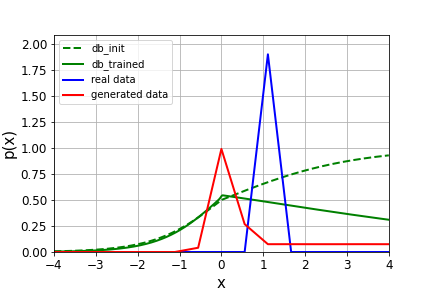
\includegraphics[width=1\linewidth]{Standard.png}} a) \\
\end{minipage}
\hfill
\begin{minipage}[h]{0.47\linewidth}
\center{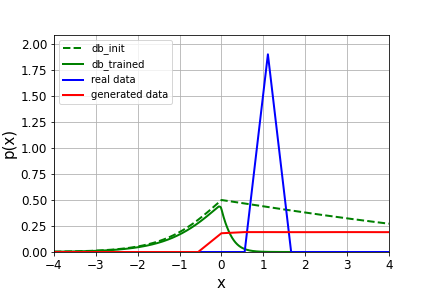
\includegraphics[width=1\linewidth]{Primal-dual.png}} \\b)
\end{minipage}
\vfill

\caption{Результаты обучения GAN в модельном эксперименте: a) для стандартного метода тренировки, b) для прямо-двойственного субградиентного метода.  }
\label{ris:experiments toy example}
\end{figure}
\begin{table}[h]
    \centering
    % \begin{tabular}{c|c}
    %      &  \\
    %      & 
    % \end{tabular}
    \begin{tabular}{|c|c|c|}
\hline 
 & Генератор & Дискриминатор \\ 
\hline 
Вход & $\mathbb{R}$ & $\mathbb{R}$ \\ 
\hline 
Скрытый слой & 32 нейрона + ReLU & 32 нейрона + ReLU \\ 
\hline 
Выход & $\mathbb{R}$  & $\sigma(\mathbb{R})$ \\ 
\hline 
\end{tabular}
    \caption{Архитектура GAN в модельном эксперименте}
    \label{tab:my_label}
\end{table}

\subsection{Эксперимент с MNIST}

В данном разделе приведены результаты тестирования предложенного метода на датасете MNIST. Размер обучающей выборки -- 60 000 сэмплов. На Рис. 2 представлены изображения, которые генерирует GAN в результате обучения.% Мы сравниваем работу обоих методов -- стандартного и прямо-двойственного. 
В результате обучения обоими методами GAN генерирует сопоставимые по качеству изображения.
Архитектура нейросетей также представлена в Таблице 2.

\begin{table}[h]
    \centering
    % \begin{tabular}{c|c}
    %      &  \\
    %      & 
    % \end{tabular}
    \begin{tabular}{|c|c|c|}
\hline 
 & Дискриминатор & Генератор \\ 
\hline 
Вход & Картинка ($28 \times 28 \times 1$) & Массив из $\mathbb{R}^4$ \\
\hline 
Слой 1 & Conv2D ($14 \times 14 \times 128$) & Dense 3136\\ 
\hline 
Слой 2 & Leaky ReLU  & Dropout 3136 \\ 
\hline 
Слой 3 & Dropout & Reshape ($7 \times 7 \times 64$) \\
\hline
Слой 4 & MaxPooling 2D ($7 \times 7 \times 128$) & UpSampling2D ($14 \times 14 \times 64$) \\
\hline
Слой 5 & Conv2D ($7 \times 7 \times 128$) & Conv2D ($14 \times 14 \times 64$)\\
\hline
Слой 6 & Leaky ReLU & Dropout ($14 \times 14 \times 64$)\\
\hline
Слой 7 &Dropout & Conv2D ($14 \times 14 \times 32$)\\
\hline
Слой 8 & Flatten 6272& Dropout ($14 \times 14 \times 32$) \\
\hline
Слой 9 & -& UpSampling2D ($28 \times 28 \times 32$) \\
\hline
Выход & Dense $ \left( \{0,1\} \right)$ & Conv2D ($28 \times 28 \times 1$) \\
\hline
\end{tabular}
    \caption{Архитектура GAN в эксперименте MNIST}
    \label{tab:my_label}
\end{table}

\begin{figure}[h]
\begin{minipage}[h]{0.47\linewidth}
\center{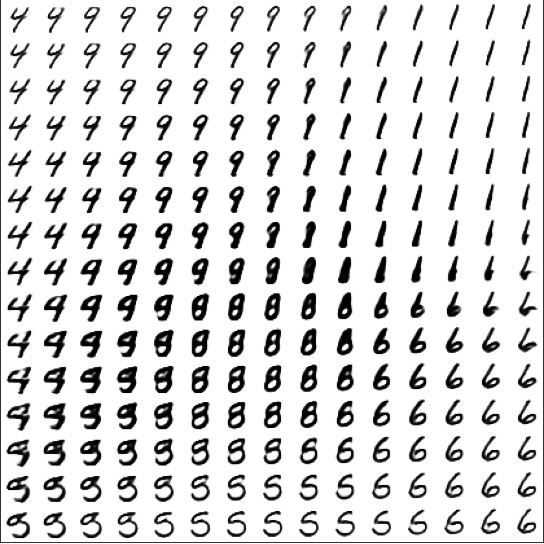
\includegraphics[width=1\linewidth]{standartny (1).jpg}} a) \\
\end{minipage}
\hfill
\begin{minipage}[h]{0.47\linewidth}
\center{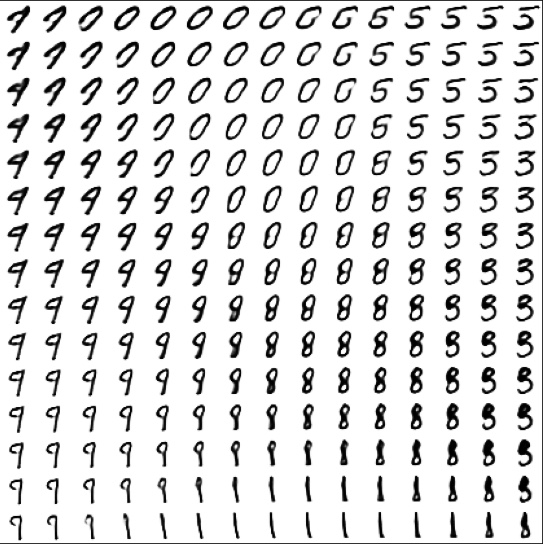
\includegraphics[width=1\linewidth]{prdv (1).jpg}} \\b)
\end{minipage}
\vfill

\caption{Результаты обучения GAN в случае тренировки a) стандартным методом, b) прямо-двойственным субградиентным методом. }
\label{ris:experiment mnist}
\end{figure}



\section{Заключение}
В данной работе проведено тестирование предложенного в статье  \cite{chen2018training} прямо-двойственного метода на задаче, в которой истинные данные распределены как $ x  \thicksim \mathcal{N} (1, 10^{-3}) $. 
Как видно из Рис. 1, в результате обучения с помощью прямо-двойственного субградиентного метода GAN начинает генерировать данные, распределение которых значительно отличается от истинного. Мы пока не знаем, как интерпретировать полученный результат. 
По какой-то причине субградиентный прямо-двойственный метод в случае гауссовского распределения ($x \thicksim \mathcal{N} (1, 10^{-3}) $) оказывается менее предпочтительным с точки зрения качества в сравнении с градиентным спуском. 
Нашей возможной дальнейшей задачей может быть изучение границ применимости предложенного в статье \cite{chen2018training} метода. 
Также интересен вопрос выбора оптимизатора, который мы в данной работе не затрагиваем. Важным направлением дальнейшней работы является попытка дать интерпретацию Алгоритму 1 (см. раздел 3).
\label{S:5}
 
\bibliographystyle{elsarticle-num-names}
\bibliography{lib.bib}

\cite{chen2018training}
\cite{lu2018understand}
\cite{goodfellow2014generative}

\end{document}
